\part{Introduction}

\chapter{Introduction}

What has been one of the main dangers humanity has faced throughout its history? The first answers that can be given are war or climate change, but there is another great threat that has severely affected the lives of almost all human populations over time: diseases and epidemics. There were no periods - not in the past, nor nowadays - when illnesses didn't influence human lives. 

Looking at the past, the consequences of epidemics on the population were worse than today, mostly because of the lack of knowledge about medical science and the poor hygienic conditions. During the bubonic plague of the 14th century, for example, 25 million deaths were reported in Europe out of a population of 100 million. The pandemic also triggered social unrest: Jews were considered responsible for the illness spread and they began to be persecuted: there were several attacks and massacres to the Jewish communities in different European cities, like Toulon, Barcelona, Erfurt, Basel, Frankfurt, Strasbourg. The persecution mainly was related to belief that Jews were less affected by the disease, and that were responsible of the poisoning of wells.
\begin{figure}[ht]
	\centering
	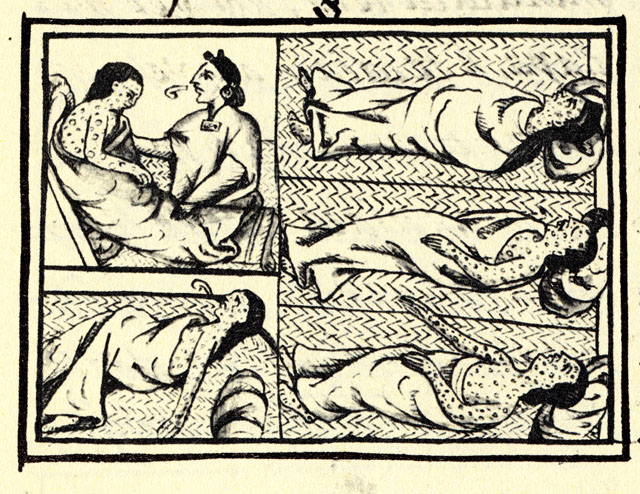
\includegraphics[width=0.43\linewidth]{0_introduction/images_introduction/FlorentineCodex_smallpox}
	\caption[Smallpox on native Americans]{Representation of smallpox disease on the Mexican population in the $XIV$ century. Figure from the Florentine Codex \cite{Sahagun1965}. }
	\label{fig:florentinecodexsmallpox}
\end{figure}
\\
\newpage
Another example is how during the course of the Americas' colonization, the diseases imported by the Europeans were one of the main causes of the genocide of the local population, largely contributing to their defeat against the Spanish conquistadors. In fact, diseases like smallpox and cholera were unknown in these countries and native Americans had no antibodies to contrast them. 
Other important epidemics, famous for their consequences, were the Spanish influenza, Smallpox, Typhus, HIV/AIDS, and the more recent COVID-19. 
It is straightforward to notice the effect that diseases have on our lives.

The development of modern medicine and hygiene contributed to enhancing the quality of life. An example of this is that only in the last three centuries and especially in the most economically developed countries, a significant increase in life expectancy has been observed \cite{Anderson_82}.
This increase is also happening in poorer regions, such as Sub-Saharan Africa. Although their current life expectancy is lower than that of wealthier countries, recent research \cite{Vollset_2024} predicts a significant rise over the next 30 years. This study also forecasts that this trend will lead to a global convergence in life expectancy between now and 2050.
The most plausible explanation for this future prediction is that improvements in healthcare levels lead to changes in the causes of mortality as nations' wealth increases. In poorer regions, the primary causes of death are communicable, maternal, neonatal, and nutritional diseases, whereas in more developed and wealthier countries, non-communicable diseases like cancer and cardiovascular conditions become the main causes of death \cite{eurostat}.

However, despite rising life expectancy, epidemics continue to be one of the most significant threats to populations. In fact, there was a notable increase in the frequency and magnitude of reported epidemics during the 19th and 20th centuries \cite{Anderson_82}. This makes it essential to develop effective policies to control and mitigate their impact, requiring coordinated implementation by countries within the same macro-region.
\begin{figure}[h]
	\centering
	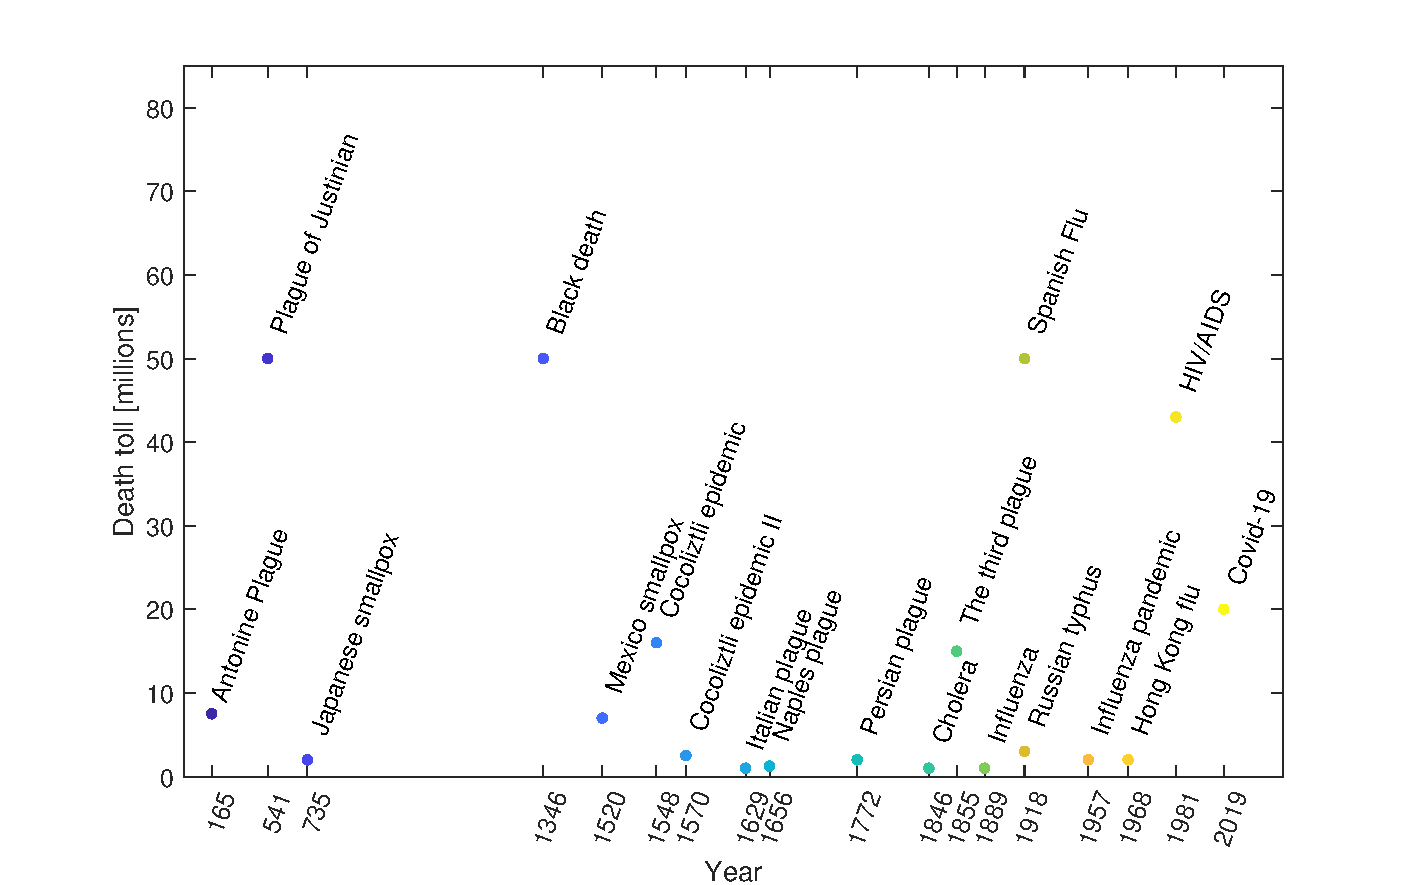
\includegraphics[width=0.95\linewidth]{0_introduction/images_introduction/worst_epidemic}
	\caption[Epidemic distribution in time]{A graphical representation of the distribution of known epidemics over the years and of their associated death toll. It is observable how there is an increment in the number of these event in the last three centuries. Data extracted from \cite{owid_historical_pandemics,wiki_pandemics}}
	\label{fig:worstepidemic}
\end{figure}

Figure \ref{fig:worstepidemic} highlights this trend. Although it becomes increasingly difficult to obtain reliable information about disease outbreaks the further back in time one goes, epidemics remain a tangible and present threat. This underscores the need for attention and action in shaping health policies that effectively address these dangers.
However, health status is not the only factor impacted by diseases. Illness can profoundly alter relationships, work, and social life, leading to a deterioration in overall social well-being as well \cite{Yang_2020}. 
There is also an economic cost associated with the cure. Only in a few nations worldwide, is treatment covered free of charge by the state. In the majority of countries, being ill can result in having to sustain high costs, causing people to go into debt or not take care \cite{esteban_2017, Barlow2021}. 
All these effects sum together and influence how populations behave when facing an epidemic. What are the consequences of adopting a certain behavior during a disease outbreak? It's a crucial question that can help to understand how to develop more efficient policies for contrasting epidemics. It is also the question that represents the first objective of study for the present work: How can a multidisciplinary model be developed that integrates elements from both social and epidemiological aspects to provide some insights into their mutual influence during the spread of a disease?
\\
\newline
Taking a step back, it's important to understand why epidemic models are crucial and what this field of research entails.
When a new disease emerges, the primary objective is to develop a defense against it. This begins with an epidemiological investigation to understand the disease's origin, the biological mechanisms behind its spread, and its resistance to existing drugs. The goal of this investigation is to gather all available information and understand the unfolding situation.
The next crucial step involves studying the dynamics of the disease and developing a predictive model for its evolution. This process requires understanding and estimating various parameters associated with the disease, including the transmission mechanisms within the population, the reproductive rate of the infectious agent, the acquisition and persistence of immunity, and the contagion mechanism.
Creating a reliable model is not only scientifically valuable but also serves as a powerful tool for stakeholders, helping to formulate effective policies during a pandemic emergency. Theoretical epidemiology aims to provide insights and policy recommendations in this context. Furthermore, data acquisition and analysis are essential for statistically modeling epidemic coefficients. 
Ultimately, a model that can address stakeholders' questions and make predictions—whether or not safety regulations are implemented—has significant implications for society. Beyond the economic costs associated with illnesses, there are also substantial social costs. Developing tools to understand better disease transmission can help mitigate its impact and alleviate the social burden, potentially saving numerous lives.
\\ \newline
A clear example of the potential benefits of having an epidemic model is the ability to generate synthetic insights that are easy to understand and can be expressed numerically. Such models can provide answers to critical questions like:
\begin{itemize}
	\item Is the disease so infective that can cause a pandemic?
	\item What are the threshold conditions that can cause an outbreak? 
	\item What is the expected number of infections over time?
\end{itemize}

At first glance, the problem may appear straightforward. However, the creation of a model capable of evaluating every disease remains an unsolved challenge.
Research in epidemic modeling requires striking a balance between simplification and maintaining accuracy. A good model effectively reproduces key phenomena with reasonable sophistication. While creating an overly complex model that attempts to incorporate every detail of a disease might be tempting, it often requires significant effort and data. In many cases, such models don't outperform simpler ones that focus on capturing the most important dynamics of disease spread. By prioritizing essential characteristics, simpler models can provide more practical insights while remaining computationally efficient.

Over the past century, various aspects of epidemics have been extensively studied. Notable achievements by scientists include:
\begin{itemize}
	\item Development of epidemiological models using different mathematical tools, such as differential equations, networks or agent-based models \cite{Hernandez_Vargas_2022, Keeling_2005}.
	\item Predictions about the progression of epidemics or reconstructions of the events' dynamics \cite{diekmann2000mathematical, brauer2012mathematical, Ledder_2023}.
	\item Insights into epidemics, explaining phenomena like the periodicity of re-infection for certain diseases or the seasonal patterns observed in cases such as influenza \cite{Bjoernstad2016}.
	\item Understanding the effectiveness of specific strategies against outbreaks, such as vaccines or quarantines \cite{Wang_2015_review}.
\end{itemize}
Furthermore, by using multilayer networks or systems, more complex analyses can be performed. The objective is to create models capable of simulating the evolution of multiple phenomena simultaneously or to develop a more accurate representation of the real world by constructing more intricate scenarios. Examples of such models include:
\begin{itemize}
	\item The simultaneous evolution of two different diseases \cite{DeDomenico2016}.
	\item The formation of public opinions during an outbreak \cite{teslya2022}.
	\item The progression of a disease for which a vaccine exists, but where there is public fear of both the disease and potential vaccine side effects \cite{Epstein_2021}.
\end{itemize}

\section{Presentation of the work realized}
The work presented in this thesis is part of the multidisciplinary field of research. Its focus lies in understanding the mutual influence between human behavior and an epidemic. On the one hand, it examines how the presence of an epidemic affects individuals' behavior; on the other hand, it explores how these behavioral changes influence the progression and dynamics of the epidemic itself.

For this reason, a new model has been developed, drawing from studies of existing multi-system models and from empirical data that integrate both epidemic and behavioral aspects.

The framework involves coupling a SIR-like disease model with a new behavioral model consisting of three compartments: Heedless, Against, and Compliant individuals. These categories are designed to represent different courses of action taken during a disease epidemic.
\begin{itemize}
	\item The Heedless individuals represent the segment of the population that is either unaware of the disease’s spread, particularly in its early stages, or indifferent to the risks, continuing with regular routines that may increase their likelihood of infection.
	\item The Against group includes skeptics who reject precautionary measures and refuse to follow established guidelines.
	\item The Compliant group consists of those who actively seek to avoid infection by adhering to health policies and precautions.

\end{itemize}

The model incorporates mechanisms to account for changes in behavior among social groups, primarily driven by peer pressure, but also considers the intervention of a central global actor. Additionally, it accounts for fatigue associated with adhering to a particular behavioral spectrum (either complying with or opposing rules). The epidemiological model developed can track both the initial phase of an epidemic and successive waves of contagion, including the possibility of reinfection.

A distinguishing aspect of this work is its reliance on empirical data. Unlike other studies that use ad-hoc assumptions or data from sources not directly related to behavior (such as opinions), this thesis leverages research conducted during the COVID-19 pandemic. This research provides insights into people's behavior, including opinions about the disease, trust or distrust in doctors or governments, and actions such as mask-wearing and handwashing.

For a novel multi-system model such as the one developed here, an analysis of its dynamics is performed. The two components alone have been studied, and the social one, which represents a novelty, has been thoroughly analyzed and simulated.
Furthermore, an epidemic reproduction number, defined as $E_0$ in the thesis, is calculated and used to understand which model-free disease scenarios can evolve into an epidemic if perturbed by the entry of infected individuals.

A powerful feature of multi-system models is their ability to reveal phenomena that would not be apparent when examining individual components in isolation. This comprehensive approach enables a deeper understanding of complex interactions and dynamics. Moreover, the developed model is designed as a flexible framework, capable of adapting to a wide range of scenarios, reflecting the multiplicity of reality. 

